\documentclass[11pt]{article}

\usepackage[utf8]{inputenc}
\input{glyphtounicode}
\pdfgentounicode=1
\usepackage{amsmath,amssymb}
\usepackage{booktabs}
\usepackage{xcolor}
\usepackage{graphicx}
\usepackage{hyperref}
\usepackage[margin=1in]{geometry}
\usepackage{url}
\def\UrlBreaks{\do\/\do-\do_}

\hypersetup{colorlinks=true, linkcolor=blue, citecolor=blue, urlcolor=blue}
\setlength{\tabcolsep}{4pt}
% Open items of this draft are marked in red; none of them is a result.
\newcommand{\todo}[1]{\textcolor{red}{[TODO: #1]}}

\title{Readable Depth Without the Calibration Map:\\
Formula Placement on Heavy-Hex Devices, and a Defect the Calibration Does Not Show}

\author{TN Holdings\\
\texttt{love.os.architect@proton.me}\\
\texttt{https://github.com/TN-Holdings-LLC/psf-zero}}

\date{Version 1.1 --- 31 October 2026}

\begin{document}
\maketitle

\begin{abstract}
Compilers for today's quantum processors choose a layout by reading the day's calibration: error rates per qubit
and per coupler. A classical computer offers no such map, and a map is stale as soon as it is read. We ask how deep a
circuit stays readable when no placement reads a quality number. We place a ring of CZ gates on IBM's heavy-hex
devices in three ways that see only the coupling graph, the basis and which elements have failed: a formula that puts
the ring on a lattice cycle (the \emph{rule}), the ring folded onto the same qubits (\emph{zipper}), and Qiskit's
level-2 search given the coupling map without error rates (\emph{blind Qiskit}). As the workload we use the kicked
Ising ring at $J=\pi/4$, whose exact answer is known at any size, and as the probe a weight-2 charge conserved by the
circuit itself: its decay, read with a four-input combination that cancels readout and first-order relaxation, gives
the per-step damping without any calibration data. In declared tests on \texttt{ibm\_marrakesh} and
\texttt{ibm\_kingston} (29 October 2026; $n=20$ and $36$; $L=24$, $50$, $100$ steps, up to 3600 CZ per circuit) the
rule kept more of the charge than both other placements in all 24 comparisons. Its readable depth, the $1/e$ decay
length $L^*$, was 56--57 steps on marrakesh and 81--90 on kingston, against 15--26 for the others: 30--73 steps
deeper. In an earlier test with a 16-layer classifier at $n=13$--$24$ the rule beat blind Qiskit at 11 of 12 sizes
and tied one. The noise model we declared did not hold: one depolarizing rate did not describe the decay on either
device, and the zipper's penalty, 3.5--3.7 times the rule's decay rate on both devices, was larger than its gate count
and duration predict (2.2--2.4). A second day (30 October) added a mirror echo of the same ring with a longitudinal
field that breaks integrability, sizes up to $n=72$ and the global parity. The rule's lead survived: 71 wins, 11 ties
and no loss in 144 comparisons (62 not judged, both arms at the noise floor). The penalty fixed after the first day
did not carry over to the echo (zipper ratio 1.7--2.7 against $3.3$--$3.9$), and the declared parity volumes were too
optimistic. On \texttt{ibm\_kingston} the rule's $n=40$ ring carried a run of 18 sites whose echo was near random or
inverted, the same 18 sites in three runs of the byte-identical circuit over three hours, while the calibration showed
nothing there and the same qubits were healthy on the $n=20$ ring. Gate twirling, which leaves the ideal circuit
unchanged, turned the inverted part random: the cause is on the device, not in the circuit. These sites set the
readable depth at $n\ge40$ (13--16 steps against 22--26 at $n=20$, 36) and erased the parity at $n=40$. A map read
from the calibration could not have avoided them. On \texttt{ibm\_fez} the next day, the byte-identical $n=20$
circuit, healthy in three runs on kingston, lost 11 of its 20 sites: the dead runs follow the chip, not the circuit.
\end{abstract}

\section{Introduction}

\begin{itemize}
\item Map-aware placement is the default (Qiskit's VF2 post-layout and noise-aware routing read error rates). Its
  gains are measured against the same map that chose the layout; the selection is optimistic by construction (the
  optimizer's curse \cite{smith2006}), and the map ages.
\item The question here: without any quality number, how deep can a circuit be read, and does the placement change
  that depth? We call a placement \emph{map-free} if it reads only the coupling graph, the basis and the failed
  elements. Map-aware placement is a special condition and is always labelled so.
\item What is new: (i) a map-free comparison of placements by a calibration-free decay measurement on the circuit
  itself; (ii) the readable depth $L^*$ and the gain $\Delta L$ as the reported quantity; (iii) declared predictions,
  with the failed ones reported. What is not new: reading noise from conserved quantities
  \cite{maruyoshi2023,oliva2026}, layer fidelity and size-independent layer errors \cite{mckay2023}, the noisy
  free-fermion solution \cite{pocklington2026}, and the $J=\pi/4$ kicked Ising circuit on IBM devices \cite{fischer2024}.
\item A picture from underwater acoustics guides the reading (Section~\ref{sec:acoustic}). Sound in the ocean fades
  with distance at a rate set by its frequency and by the water; low tones in the deep sound channel carry for
  thousands of kilometres. Here the depth of a circuit plays the distance, the Pauli weight of what is read plays the
  frequency, the placement plays the water, and a conserved charge plays the sound channel. It is an analogy for the
  reader, not a physical identity.
\item Companion work: the formula schedules and their gate counts \cite{paper4}.
\item Second day (30 October): a non-integrable mirror echo, sizes to $n=72$, the global parity, and a defect that
  no calibration number shows (Sections~\ref{sec:echo}--\ref{sec:parity}).
\end{itemize}

\section{Setting}

\subsection{Workload}
The kicked Ising ring, one step $S=(R_X(2h)\,Z)^{\otimes n}\,\mathrm{CZ}_{\mathrm{ring}}$, $J=\pi/4$, $h=0.6$. It is a
free-fermion circuit; its outputs are computed exactly at any $n$ by a recursion, which also gives the outputs under
uniform depolarizing noise exactly \cite{pocklington2026}. With the Jordan--Wigner transformation in the $X$ basis,
one step is a Gaussian unitary of the $2n$ Majorana operators: their covariance matrix $\Gamma$ evolves as
$\Gamma\mapsto R\,\Gamma R^{\mathsf T}$ with a fixed orthogonal $2n\times2n$ matrix $R$, so any quadratic quantity after
$L$ steps costs $O(n^3)$ and no state vector is needed at any $n$ (TOQB's \texttt{toqb.kising}, checked against a state
vector at small $n$). The probes below need even less: P1 uses only that the charge is conserved, and P3
(Section~\ref{sec:echo}) only that its circuit is the identity up to a known flip.

\subsection{Placements (no quality number read)}
\begin{itemize}
\item \textbf{Rule} (\texttt{fold:rule}): the ring on a cycle of the heavy-hex lattice, built by formula from the
  lattice's cells \cite{paper4}; $n$ CZ per layer.
\item \textbf{Zipper} (\texttt{fold:zipcyc}): the ring folded onto the same cycle's qubits; $5n/2-4$ CZ per layer.
\item \textbf{Blind Qiskit} (\texttt{qiskit:2:blind:template}): Qiskit level 2, \texttt{seed\_transpiler}=0, given the
  working couplers in both directions and the basis only.
\item Failed elements (error $=1$) are removed for every placement; nothing else of the calibration is used.
\end{itemize}

\subsection{Probe P1: the circuit's own conserved charge}
\[
Q=\sum_j \bigl(Z_jZ_{j+1}+b\,Y_jZ_{j+1}+c\,Z_jY_{j+1}\bigr),\qquad b=c=-1.28608\ (h=0.6),
\]
the weight-2 conserved charge with the largest $ZZ$ share (a noiseless criterion; the same coefficients for
$n=6$--$40$). Inputs $|0\cdots0\rangle$, $|1\cdots1\rangle$ and the two N\'eel states; three measurement settings;
every record carries its own readout reference on the physical qubits it measures. The four-input ratio
\[
\rho(L)=\frac{[Q(0\cdots0)+Q(1\cdots1)-Q(\text{N\'eel})-Q(\overline{\text{N\'eel}})]_L}{[\,\cdot\,]_{\mathrm{ref}}}
\]
cancels readout within a record and the first-order relaxation bias. Under uniform depolarizing noise
$\rho(L)=(1-4p/3)^{2L}$.

\subsection{Readable depth}
$L^*$ is the $1/e$ decay length of a one-parameter fit $\rho(L)=e^{-L/L^*}$ over $L=24,50,100$ (weighted least squares
on the $\rho$ scale). $\Delta L_X=L^*_{\mathrm{rule}}-L^*_X$ and $\kappa_X=L^*_{\mathrm{rule}}/L^*_X$, the ratio of
per-step decay rates. $L^*$ is a property of a weight-2 quantity; wider outputs decay faster (Section~\ref{sec:p2}).

\subsection{An acoustic reading of the decay}\label{sec:acoustic}
Under uniform depolarizing noise of rate $p$ per qubit and step, a Pauli string of weight $w$ is multiplied by
$(1-4p/3)^{w}$ at every step. The attenuation per step therefore grows with the weight, as the absorption of sound in
sea water grows with frequency \cite{francois1982}. Table~\ref{tab:acoustic} lists the correspondence we use.

\begin{table}[h]
\centering
\small
\begin{tabular}{p{0.36\textwidth}p{0.58\textwidth}}
\toprule
sound in the ocean & a circuit on a device\\
\midrule
distance travelled & depth $L$ (steps)\\
absorption coefficient; attenuation length & per-step decay rate; $L^*$\\
frequency (higher tones fade sooner) & Pauli weight of the observable (wider observables fade sooner)\\
the water (temperature, salinity) & the placement (the zipper absorbs about 3.6 times as much as the rule)\\
geometric spreading loss & operator spreading: a local output grows in weight before the noise acts on it\\
the deep sound (SOFAR) channel & a conserved charge: the circuit does not spread it; only the noise damps it\\
sonar equation and detection range & signal against shot noise; the readable depth at a shot budget\\
\bottomrule
\end{tabular}
\caption{The analogy used in this paper. Where it fails: sea-water absorption grows roughly as the square of the
frequency, with relaxation peaks, and is an empirical formula; the weight dependence here is linear in the exponent
and follows from the noise model.}\label{tab:acoustic}
\end{table}

In the language of the sonar equation \cite{urick1983}, a reading at depth $L$ is detected when the signal exceeds
twice its shot-noise standard error. With $\rho(L)=e^{-L/L^*}$ and a per-shot spread $\sigma_1$ (so that
$\mathrm{SE}=\sigma_1/\sqrt{S}$ at $S$ shots),
\[
L_{\mathrm{read}}(S)=L^*\,\ln\frac{\sqrt{S}}{2\sigma_1}.
\]
For probe P1, $\sigma_1\approx0.2$--$0.26$, so $L_{\mathrm{read}}(1000)\approx4L^*$. That lies beyond the depths we
measured and is not claimed; we report $L^*$, which needs no budget and no threshold. The formula does show why the
gain matters: $\Delta L$ in $L^*$ becomes about four times as many steps of detection range at 1000 shots, and a
placement that absorbs $\kappa$ times as much reaches $\kappa$ times fewer steps with the same shots.

\subsection{Declarations}
Every device test was declared (SHA-256 and CET time) before its calibration was fetched; the declarations, records
and raw counts are in TOQB \cite{toqb}; Table~\ref{tab:decl} lists them.

\begin{table}[h]
\centering
\footnotesize
\begin{tabular}{p{0.19\textwidth}p{0.3\textwidth}p{0.45\textwidth}}
\toprule
test (device, date) & declaration (SHA-256) & jobs\\
\midrule
D6 (kingston, 28 Oct) & \texttt{device\_d6\_note} (85b358b7) & \texttt{dbh0s6sdgr2s73csfnrg}\\
noise wall (marrakesh, 29 Oct) & \texttt{noise\_wall\_1\_second\_device\_note} r2 (d963adb6) & \texttt{dbhhsncdgr2s73ctiung} (P1), \texttt{dbhhuc9t9uhs73ca9t70} (P2)\\
noise wall (kingston, 29 Oct) & \texttt{noise\_wall\_1\_note} r3 (7415beca) & \texttt{dbhiji1t9uhs73cab78g} (P1), \texttt{dbhil0kdgr2s73ctkd20} (P2)\\
test 2 (both, 30 Oct) & \texttt{echo\_hz\_note} (1308cf9b), addendum 1 (a206c81a) & \texttt{dbi7pmg1h92s7382ubkg}, \texttt{dbi7r45ep8hs73anb5q0}\\
test 3 (both, 30 Oct) & \texttt{test3\_note} (8b13773f), addenda 1, 2 (1c484fa8, 78986cf3) & marrakesh \texttt{dbi7qg6ne4hc73be2nf0}, \texttt{dbi7qig1h92s7382ucn0}, \texttt{dbi7qkmne4hc73be2njg}; kingston \texttt{dbi7rtene4hc73be2p8g}, \texttt{dbi7rvune4hc73be2pcg}, \texttt{dbi7s1tep8hs73anb72g}\\
rule-only rerun (kingston, 30 Oct) & \texttt{rerun\_rule\_only\_note} (1f883a77) & \texttt{dbi9fhene4hc73be4u50}\\
options test (kingston, 30 Oct) & \texttt{options\_test\_note} (2ebd84e2) & \texttt{dbiah1ghoj4c73b5qkrg} (off), \texttt{dbiah38hoj4c73b5qku0} (DD), \texttt{dbiah581h92s73832mh0} (twirling)\\
rule-only echo (fez, 31 Oct) & \texttt{fez\_rule\_only\_note} (6011c240) & \texttt{dbilc0ghoj4c73b6fkq0}\\
\bottomrule
\end{tabular}
\caption{Declarations, fixed before each test's calibration fetch, and the IBM job identifiers.}\label{tab:decl}
\end{table}

\section{Classifier test without the map (D6)}
TOQB's ring classifier, $L=16$, $n=13$--$24$, 64 inputs $\times$ 250 shots, \texttt{ibm\_kingston}, 28 October 2026;
no arm read a quality number and no simulator was used. Rule against blind Qiskit: 11 wins, 1 tie (at $n=23$), no
loss. Rule against the zipper on the same qubits (even $n$): 3 wins, 3 ties, no loss. Blind Qiskit kept no measurable
signal at 8 of 12 sizes; its circuits ran 22--108\,\textmu s against the rule's 5.6--9.3\,\textmu s.
For reference, with the map (D5 part A, $n=20$, a different hour): rule $0.943\pm0.044$, zipper $0.600\pm0.044$,
map-aware Qiskit $0.765\pm0.099$ (rule $-$ Qiskit within 2 SE). Table~\ref{tab:d6} gives the slopes.

\begin{table}[h]
\centering
\small
\begin{tabular}{lccc|lccc}
\toprule
$n$ & rule & zipper & blind Qiskit & $n$ & rule & zipper & blind Qiskit\\
\midrule
13 & $0.78\pm0.11$ & -- & $0.38\pm0.11$ & 19 & $0.78\pm0.11$ & -- & $0.37\pm0.14$\\
14 & $0.75\pm0.08$ & $0.61\pm0.10$ & $-0.08\pm0.22$ & 20 & $0.83\pm0.07$ & $0.69\pm0.06$ & $0.49\pm0.11$\\
15 & $0.90\pm0.08$ & -- & $0.00\pm0.07$ & 21 & $0.85\pm0.09$ & -- & $0.08\pm0.10$\\
16 & $0.85\pm0.09$ & $0.48\pm0.09$ & $-0.02\pm0.11$ & 22 & $0.69\pm0.12$ & $0.32\pm0.13$ & $0.09\pm0.10$\\
17 & $0.91\pm0.08$ & -- & $-0.07\pm0.10$ & 23 & $0.37\pm0.15$ & -- & $0.00\pm0.21$\\
18 & $0.58\pm0.09$ & $0.50\pm0.09$ & $0.05\pm0.14$ & 24 & $1.00\pm0.13$ & $0.38\pm0.11$ & $0.41\pm0.14$\\
\bottomrule
\end{tabular}
\caption{D6: the classifier's device slope $\lambda$ ($\pm$ SE; 64 inputs $\times$ 250 shots), \texttt{ibm\_kingston},
28 October 2026. The zipper exists for even $n$ only.}\label{tab:d6}
\end{table}

\section{The noise wall on two devices}

\begin{table}[h]
\centering
\small
\begin{tabular}{lcccc}
\toprule
 & marrakesh $n=20$ & marrakesh $n=36$ & kingston $n=20$ & kingston $n=36$\\
\midrule
$L^*$ rule & $56.5\pm0.9$ & $56.6\pm0.7$ & $81.3\pm1.3$ & $89.7\pm1.1$\\
$L^*$ zipper & $15.1\pm0.4$ & $15.7\pm0.3$ & $22.6\pm0.4$ & $25.6\pm0.3$\\
$L^*$ blind Qiskit & $26.4\pm0.5$ & $15.7\pm0.3$ & $22.0\pm0.4$ & $17.0\pm0.3$\\
$\Delta L$ vs zipper & $+41.3$ & $+40.9$ & $+58.7$ & $+64.1$\\
$\Delta L$ vs blind Qiskit & $+30.1$ & $+40.9$ & $+59.3$ & $+72.7$\\
$\kappa$ zipper ($g$, $t$) & 3.73 (2.30, 2.27) & 3.60 (2.39, 2.25) & 3.60 (2.30, 2.24) & 3.50 (2.39, 2.22)\\
rule wins on $\rho$ & 6/6 & 6/6 & 6/6 & 6/6\\
\bottomrule
\end{tabular}
\caption{Probe P1 on two devices, 29 October 2026. $g$, $t$: the zipper's gate and duration ratios to the rule. 1000 shots per circuit; jobs of 92 and 90\,s.
Full tables in TOQB's result folders.}
\end{table}

\begin{itemize}
\item \textbf{Benchmark number:} the rule won all 24 charge comparisons; $\Delta L=+30$ to $+73$ steps.
\item \textbf{Device user's number:} at $n=36$, $L=100$ (3600 CZ) the rule's charge was $0.178\pm0.006$ (marrakesh)
  and $0.314\pm0.006$ (kingston); the zipper's and blind Qiskit's were zero within 2 SE.
\end{itemize}

\section{Declared predictions that failed}
\begin{itemize}
\item \textbf{One depolarizing rate.} Neither device followed $\rho=(1-4p/3)^{2L}$ with one $p$ within 2 shot-noise
  SE: marrakesh against its own $p$ from $L=24$ (1 of 5 inside), kingston against $p=0.0051$ from the previous day
  (1 of 6). The per-segment decay rates scatter by 10--20\,\% with no common direction, and kingston's rate had
  improved since the previous day; the declared tolerance (shot noise only, about 1\,\%) left no room for either.
\item \textbf{Size independence of the rule.} SAME at all three depths on marrakesh; DIFFERENT at $L=24$ and 50 on
  kingston, where the $n=36$ ring was better than the $n=20$ ring.
\item \textbf{The structure bracket.} The zipper's $\kappa$ was declared to lie between its gate ratio and its
  duration ratio (2.2--2.4). It was 3.5--3.7 on both devices.
\item \textbf{Probe P2} ($\langle X_0\rangle$, 250 shots) was at the noise floor on both devices.
\end{itemize}

\section{The formula fixed after the run}\label{sec:fixed}
The following changes were made after seeing the results. They are fitted to the same data and are evidence only once
they predict a later run; they are declared for the next stage.
\begin{enumerate}
\item \textbf{Self-reference with a model band.} The rule's rate is read from its own $L=24$ point; deeper points are
  predicted with the rate $\pm20$\,\% (the observed scatter), plus 2 SE of shot noise.
\item \textbf{A constant zipper penalty.} $L^*_{\text{zipper}}=L^*_{\text{rule}}/3.6$, with $\kappa\in[3.3,3.9]$,
  in place of the structure bracket.
\item \textbf{Map-aware, for reference only (special condition).} $1/L^*=c\times$ the median CZ error of the rule's
  couplers on the day's calibration.
\end{enumerate}

\begin{table}[h]
\centering
\small
\begin{tabular}{p{0.48\textwidth}p{0.2\textwidth}p{0.24\textwidth}}
\toprule
fixed formula & on its own data & fitted on one device, applied to the other\\
\midrule
1. own $L=24$ point, rate $\pm20$\,\% & 8/8 & (no device constant)\\
1b. $n=20$ ring's $L=24$ point to the $n=36$ ring & 6/6 & (no device constant)\\
2. zipper $\kappa=3.6\pm0.3$ & 4/4 & 4/4\\
3. map-aware: $1/L^*=c\times$ median CZ error & fits by construction & 1/4 ($-27$ to $+37$\,\%)\\
\bottomrule
\end{tabular}
\caption{The fixed formulas on 29 October 2026 (post-hoc). Formula 3 reads the calibration and failed across devices:
the day's error map did not predict the readable depth better than the circuit's own short-depth point.}
\end{table}

Formula 2 was then declared for the next day's probes. It failed on both: the zipper's ratio was 1.7--2.7 on the
echo (Section~\ref{sec:echo}) and 1.7--2.6 on the parity (Section~\ref{sec:parity}). The penalty measured on the
charge is a property of that probe, not of the placement alone.

\begin{figure}[h]
\centering
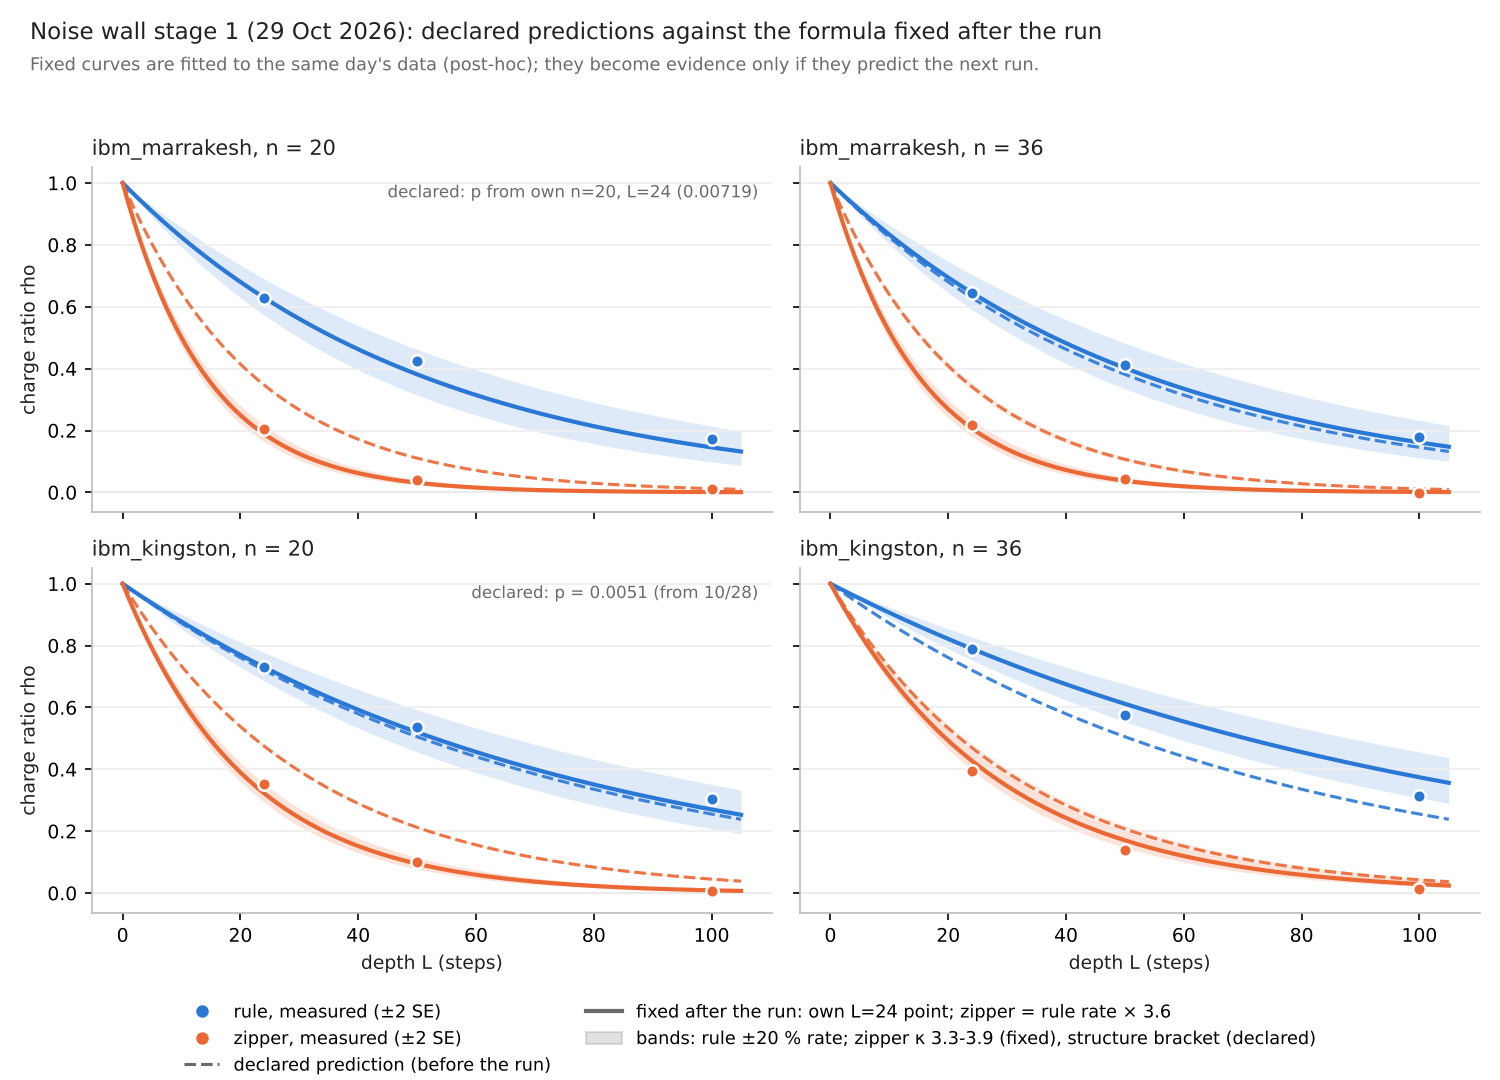
\includegraphics[width=\textwidth]{figures/readable_depth_declared_vs_fixed.png}
\caption{Declared predictions (dashed) against the formula fixed after the run (solid, with bands), for the rule (blue)
and the zipper (orange) on both devices and both sizes. Points: measured $\rho$, $\pm2$ SE. The largest miss of the
declared predictions is the zipper's: its structure ratio (about 2.3) underestimated its penalty (about 3.6) on all
four panels. Fitted to the same day's data; script \texttt{readable\_depth\_figures.py}.}\label{fig:fixed}
\end{figure}

\section{Second day: a non-integrable echo and larger rings}\label{sec:echo}

\subsection{Probe P3: the mirror echo}
The step gets a longitudinal field, $S=(R_X(2h)\,Z\,R_Z(2h_z))^{\otimes n}\,\mathrm{CZ}_{\mathrm{ring}}$, which breaks
integrability for $h_z\neq0$ and leaves the two-qubit structure unchanged ($R_Z$ commutes with the CZ ring). The echo
runs $L$ steps forward, flips every qubit ($W=X^{\otimes n}$), and runs $L$ steps of $(WSW)^{-1}$. Since
$WSW$ is $S$ with every angle negated,
\[
U=(WSW)^{-L}\,W\,S^{L}=W\,S^{-L}\,W\,W\,S^{L}=W ,
\]
so the noiseless output is the flipped input at any $n$ and $h_z$, and no simulation is needed. The flip also keeps a
compiler from cancelling the two halves. Inputs and readout reference are as for P1; the reported quantity is
$\rho_E(D)$, the four-input ratio of $\sum_j(-z_j)\langle Z_j\rangle$ to its reference, at full depth $D=2L=24$, 50,
100, and $L^*$ is its decay length in the same steps as before. P3 reads weight-1 outputs; it is not P1's charge and its
$L^*$ is not comparable with Section~5's.

\subsection{Declared tests and results}
Test 2 ($n=20$, 36) and part E of test 3 ($n=40$, 72), $h_z=0$, 0.1, 0.3, three placements, 500 shots, on
\texttt{ibm\_marrakesh} and \texttt{ibm\_kingston}, 30 October 2026; declarations fixed before the fetch.
\begin{itemize}
\item \textbf{Rule A (who keeps more):} rule against each other arm at 2 SE, judged when either exceeds 2 SE. Over both
  devices: 71 wins, 11 ties, \textbf{0 losses}, 62 not judged. The lead does not depend on $h_z$.
\item \textbf{Rule B (the fixed zipper penalty, $\kappa\in[3.3,3.9]$ from Section~\ref{sec:fixed}):} BELOW wherever it
  could be judged ($\kappa=1.7$--$2.7$, 18 cells); on marrakesh's part E the zipper sat at the noise floor in 5 of 6
  cells (not judged), and the sixth, at 2.2 SE, came out ABOVE ($5.4\pm12$).
  The penalty fixed on the charge did not transfer to the echo.
\end{itemize}

\begin{table}[h]
\centering
\small
\begin{tabular}{lcccc}
\toprule
rule's $L^*$ (P3, steps) & $n=20$ & $n=36$ & $n=40$ & $n=72$\\
\midrule
kingston, 12:22 CET & 22.8--23.7 & 23.0--23.6 & 12.8--16.1 & 14.2--15.3\\
kingston, 14:12 CET (rule only, rerun) & 21.9--22.3 & 24.5--26.2 & 13.0--16.0 & 14.6--16.0\\
marrakesh, 12:17 CET & 14.6--14.8 & 14.9--15.8 & 14.1--15.3 & 14.3--15.5\\
fez, 31 Oct 03:44 CET (rule only) & 11.2--12.1 & 16.0--16.8 & 12.5--13.8 & 12.8--13.9\\
\bottomrule
\end{tabular}
\caption{The rule's echo decay length over $h_z=0$, 0.1, 0.3. On kingston it halves from $n=36$ to $n=40$; on
marrakesh it does not depend on $n$; on fez it is short at every $n$. The rerun's declared reproduction test failed at
2 SE (12 of 21 cells agreed; differences of 0.02--0.05 in $\rho_E$), while the pattern over $n$ and over sites
repeated. Fez's declared test (no wall if $L^*$ at $n=40$, 72 lies within $\pm20\,\%$ of the mean at 20, 36): no wall at
all three $h_z$, because dead runs appear at every size there (Section~\ref{sec:defect}).}\label{tab:echo}
\end{table}

\section{A defect the calibration does not show}\label{sec:defect}

Reading $\rho_E$ per site instead of as a ring average explains the halving on kingston. Let
$a_j=\frac14\sum_{\text{inputs}}\langle -z_jZ_j\rangle$ be the raw echo signal of ring site $j$ (1 perfect, 0 random,
negative when the wrong bit is read more often than the right one). Figure~\ref{fig:defect} shows $a_j$ at $D=24$,
$h_z=0$ for three runs of the byte-identical $n=40$ circuit (QPY SHA-256 \texttt{42376e3f\ldots}) at 12:22, 14:12 and
15:24 CET, under three calibrations (11:55, 13:37 and 14:57 CET).

\begin{figure}[h]
\centering
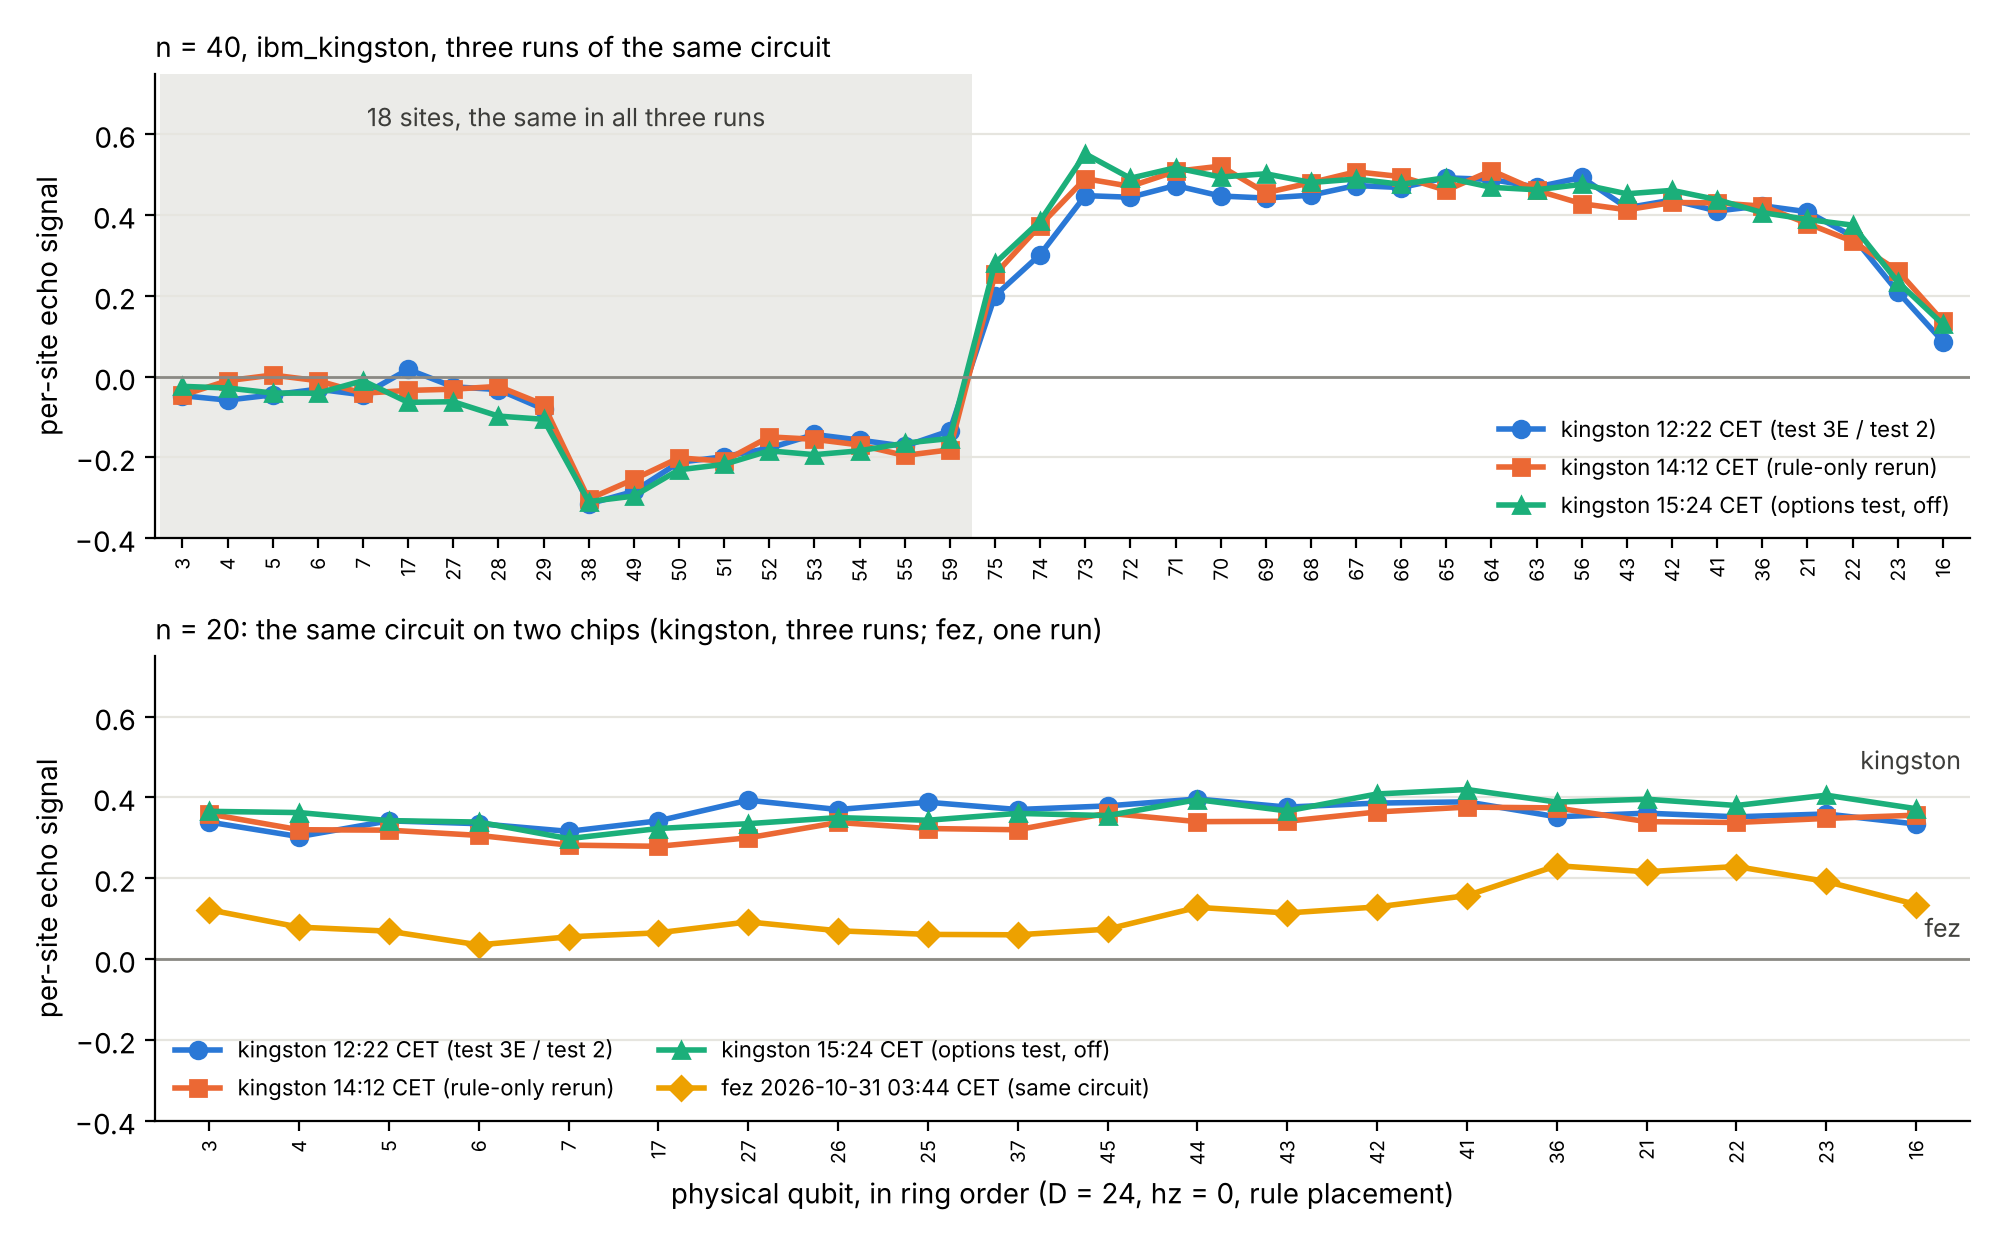
\includegraphics[width=\textwidth]{figures/defect_map_kingston_2026-10-30.png}
\caption{Per-site echo signal along the rule's ring, $D=24$, $h_z=0$. Top: $n=40$ on \texttt{ibm\_kingston},
30 October 2026, three runs of the same circuit; the shaded run of 18 sites is the same in all three. Bottom: the
$n=20$ circuit, which uses qubits 3--7, 16, 17, 27 of the same region: no such run in three runs on kingston, and on
\texttt{ibm\_fez} (31 October, the byte-identical circuit) 11 of 20 sites below 0.12. Script
\texttt{figures/defect\_map\_figure.py} on TOQB's records.}\label{fig:defect}
\end{figure}

\begin{itemize}
\item \textbf{Reproducible and localized.} The same 18 sites (qubits 3--7, 17, 27--29, 38, 49--55, 59) fell below
  $a=0.12$ in all three runs (site-wise correlation 0.98 between runs); their mean was $-0.133\pm0.004$ against
  $0.430\pm0.003$ for the other 22 (third run). Qubits 3--29 were near random, 38--59 inverted ($-0.13$ to $-0.31$).
  At $n=72$ about 31 sites in two clusters behaved the same way in two runs; at $n=20$ and 36, none.
\item \textbf{Invisible to the calibration.} On these sites the day's CZ errors were 0.001--0.009, $T_2\ge125$\,\textmu s
  and readout errors $\le1.5$\,\%; each record's own readout reference was normal there.
\item \textbf{Context-dependent.} Qubits 3--7, 16, 17, 27 are healthy on the $n=20$ ring and qubits 27--29 on the
  $n=36$ ring. The run appears when the ring passes 17--27--28--29--38. Which element or combination causes it is not
  known.
\item \textbf{Chip-specific.} The $n=20$ circuit is byte-identical on kingston and on \texttt{ibm\_fez} (QPY SHA-256
  \texttt{671db9e3\ldots}; same qubits, same gates). On kingston it had no dead site in three runs ($\rho_E=0.34$--0.40
  at $D=24$); on fez the next day (job \texttt{dbilc0ghoj4c73b6fkq0}, calibration 03:25 CET) 11 of its 20 sites were
  dead ($\rho_E=0.12$--0.14), and fez's rings of 36, 40 and 72 sites carried 6, 11 and 36. The $n=72$ circuit is also
  identical on both chips; its dead runs lie mostly in different places. The dead runs follow the chip, not the
  circuit: a second argument, independent of Lemma~1 below, that the circuit is not the cause.
\end{itemize}

Two statements about these runs can be proved rather than estimated.

\paragraph{Lemma 1 (the circuit is not the cause).} Pauli twirling of the CZ gates replaces each CZ by $P'\,\mathrm{CZ}\,P$
with $P$ a random two-qubit Pauli and $P'=\mathrm{CZ}\,P\,\mathrm{CZ}$, again a Pauli because CZ is Clifford
\cite{wallman2016}. The ideal unitary, and so the ideal output (the flipped input), is unchanged. A change of the
measured output under twirling is therefore a property of the device. Run with gate twirling (15:24 CET, otherwise
identical), the inverted part moved from $-0.214$ to $+0.015$ and the near-random part from $-0.052$ to $+0.004$; the
cause is on the device, and the inverted part is a coherent error that twirling turns into a random one. (The circuit
was also checked noiselessly at $D=2$ and 4, where every site returns the flipped input.)

\paragraph{Lemma 2 (how far one fault reaches).} Let one fault $E$ act after $t$ of the echo's $2L$ steps, so that the
noisy circuit is $U_2EU_1$ with $U_2U_1=W$. Then $U_2EU_1=W\,(U_1^\dagger EU_1)=(U_2EU_2^\dagger)\,W$. Each step moves
support by at most one site each way along the ring (nearest-neighbour CZ ring and single-qubit gates; the rule's
circuits contain no other two-qubit gates). So the effective error is supported within $\min(t,2L-t)\le L$ sites of
$E$ on either side, at most $2L+1=25$ sites at $D=24$, if errors act locally in space and time. The 18-site run at
$n=40$ fits one fault. At $n=72$ the shortest arc of the ring that holds all dead sites is 43--45 positions long (two
runs), which no single local fault can reach: there are at least two sources.

\paragraph{Options do not repair it.} Dynamical decoupling (XY4) moved the 18 sites by $+0.018\pm0.005$ and cost the
others $-0.013\pm0.004$; gate twirling moved them by $+0.143\pm0.005$ (to about zero, not back to the healthy level)
and cost the others $-0.064\pm0.004$, and the healthy $n=20$ ring a quarter of its signal (0.37 to 0.27). Neither was
kept: the standard stays without both. That decoupling, which cancels static coupling on idle qubits, does almost
nothing points away from idle crosstalk; this is a reading, not a test.

\paragraph{What the rest of the ring says.} With the dead sites taken from one run and removed from the other (both
ways, so no run is read on sites chosen from itself; post hoc), the remaining sites at $n=40$ and 72 gave
$\rho_E=0.35$--$0.45$ at $D=24$ and $L^*=18.6$--$21.3$, close to the $n=20$, 36 rings (22--26). Most of the drop with
$n$ in Table~\ref{tab:echo} sits in these runs. Masking recovers per-site quantities only; anything that needs every
bit is lost once a dead site is in it (next section).

\section{The global parity}\label{sec:parity}
$P=\prod_jX_j$ is conserved by the step at any $n$ and has weight $n$: it is the widest quantity the ring has, and one
bad site erases it. Declared (test 3, part P): the rule's volume $V^*$ in $\rho_P=e^{-nL/V^*}$ inside a band around
171 (kingston) and 113 (marrakesh), and the zipper ratio in $[3.3,3.9]$.
\begin{itemize}
\item \textbf{Failed:} the rule's $V^*$ was 72.6 and 105.8 on kingston, 59.8 and 76.4 on marrakesh ($n=20$, 36): 1 of 4
  inside. The zipper's $V^*$ was inside in 4 of 4; the ratio inside in 1 of 4 (1.7--2.6).
\item \textbf{Duels at $n=20$, 36:} rule 11 wins and 1 tie on kingston, 8 wins and 4 ties on marrakesh, no loss.
\item \textbf{Above 36:} on marrakesh the readout reference (half-filled strings) fell to about 0.1 at $n=40$ and to
  zero at $n=72$; these rings include qubits whose readout errors were 17--34\,\% in the calibration: readout ends
  the parity there. On
  kingston the reference was 0.27 at $n=40$, yet the parity was lost at $L=1$ ($-0.07\pm0.06$, against $0.54$ at
  $n=36$): the $n=40$ ring is the echo's ring of Section~\ref{sec:defect}. The longest exact ring of the day,
  $n=88$ on kingston, gave $0.22\pm0.10$ at $L=1$ (reported, not judged).
\end{itemize}

\section{Output probe P2}\label{sec:p2}
P2 was the slope $\lambda$ of $\langle X_0\rangle$ after $L=24$ and 50 steps (64 inputs $\times$ 250 shots), declared as a
second reading of the same placements. On both devices it sat at the noise floor: the rule's slopes were
$0.00$--$0.24$ with SE 0.02--0.06, without order in depth or placement (marrakesh: 0.046, 0.073, 0.004, 0.127;
kingston: 0.061, 0.027, 0.236, $-0.008$ for $n=20,L=24$; $n=20,L=50$; $n=36,L=24$; $n=36,L=50$). Of 16 comparisons
with the other arms the rule won 3 and lost none. The contrast with P1 is the
point of the acoustic picture: a single-site output spreads over a growing light cone and fades like a wide
operator, while the conserved charge is not spread by the circuit. P3 (Section~\ref{sec:echo}) reads single sites
too, but its mirror undoes the spreading, and it was readable to $D=24$--50.

\section{Discussion}
\begin{itemize}
\item \textbf{Depth, not width, up to $n=36$.} Below that size the limit was how deep the circuit stayed readable,
  not how many qubits it used: the rule's charge decay length was the same at $n=20$ and 36 on marrakesh (56.5,
  56.6) and longer at $n=36$ on kingston, and its echo decay length did not shrink from 20 to 36 on either device.
  Above that, on kingston, width came back in another form: a longer ring covers more of the chip and met a defect
  that shortened the readable depth (Section~\ref{sec:defect}). The quantity to report is $L^*$ per placement and
  size, read on the circuit itself.
\item \textbf{Selection and prediction.} The rule's schedules are fixed by formula; nothing is chosen as the best of
  several candidates by a calibration- or simulation-based score. For a selection of the best of $K$ candidates by an
  estimate with error scale $\sigma$, the prediction is optimistic by up to $\sigma\sqrt{2\ln K}$
  \cite{smith2006}; the analogy with the Occam bound \cite{blumer1987} is structural. This concerns the reliability of
  a prediction, not which placement keeps more signal, which we measured separately.
\item \textbf{Why the duration matters.} Blind Qiskit placed the bare ring at equal gate count, yet its charge decayed
  2--5 times faster per step than the rule's, with 5--9 times the duration. We did not separate idle decoherence
  from gate error; the durations point to the former.
\item \textbf{What a map buys.} D5 part A suggests about 0.3 in the classifier's slope at $n=20$; between jobs, not
  declared; a declared test against a map-aware arm was not run.
\item \textbf{What a map cannot see.} The defect of Section~\ref{sec:defect} sat on qubits and couplers with good
  calibration numbers and appeared only in one combination of them. A placement that reads the map would not have
  avoided it; only running the circuit showed it. For the comparison of placements this cuts both ways: at $n\ge40$ a
  placement's result also depends on whether its ring happens to pass such a site (the zipper's $n=40$ ring on kingston
  was near random almost everywhere), so wins at $n\ge40$ mix placement and the position of defects. The wins at
  $n=20$, 36, where no such run was seen, do not.
\end{itemize}

\section{Limitations}
\begin{itemize}
\item Four device days (28--31 October); one ring per size and placement. Dead runs were seen on kingston (one day, three runs) and on fez
  (one run); whether they persist over days, and how often they appear on other chips, is open.
\item The charge is a weight-2 quantity; $L^*$ is not the depth at which an arbitrary output stays readable.
\item The four-input ratio leaves a second-order relaxation bias.
\item Every reference here is classically computable; no classical-hardness claim is made.
\item The search-based comparison is Qiskit at optimization level 2 without error rates. Level 3, routers for
  commuting two-qubit gates (the CZ ring commutes) and other compilers were not tested; a stronger search could
  close part of the gap reported here.
\item Standard errors are shot noise only; drift between runs (a few per cent within one day, Table~\ref{tab:echo})
  is larger than that at our shot counts.
\end{itemize}

\section{Reproducibility}
TOQB \cite{toqb}: \texttt{results/device-d6-2026-10-28}, \texttt{results/noise-wall-1-marrakesh-2026-10-29},
\texttt{results/noise-wall-1-kingston-2026-10-29}, \texttt{results/device-2026-10-30} (tests 2 and 3, the rule-only
rerun with the post-hoc masking, the options test), \texttt{results/device-2026-10-31-fez}; declarations in
\texttt{prereg/}. Circuit files over GitHub's size limit are kept off the repository with their SHA-256.

\paragraph{Changes in version 1.1.} The rule-only echo on \texttt{ibm\_fez} (31 October, declared before its fetch):
a row in Table~\ref{tab:echo}, the item ``Chip-specific'' in Section~\ref{sec:defect}, the fez curve in
Figure~\ref{fig:defect}, its declaration in Table~\ref{tab:decl}, one sentence in the abstract, the limitation
updated. No earlier number or verdict changes.

\section*{Acknowledgments}
We acknowledge the use of IBM Quantum services for this work. The views expressed are those of the authors, and do
not reflect the official policy or position of IBM or the IBM Quantum team. The device runs used the IBM Quantum
Open Plan, including its one-time promotion of 180 minutes of runtime.

\begin{thebibliography}{99}
\bibitem{paper4} TN Holdings, ``Folding a Ring onto Heavy-Hex: Formula-Built Schedules with Provable Gate Counts, and
What Their Signal Shows on Twins and Devices'', version 1.2 (2026).
\bibitem{toqb} TN Holdings, TOQB, the test bench for PSF-Zero's training and device runs (2026).
\bibitem{smith2006} J. E. Smith and R. L. Winkler, ``The optimizer's curse: Skepticism and postdecision surprise in
decision analysis'', Management Science 52(3), 311--322 (2006).
\bibitem{blumer1987} A. Blumer, A. Ehrenfeucht, D. Haussler and M. K. Warmuth, ``Occam's razor'', Information Processing
Letters 24, 377--380 (1987).
\bibitem{maruyoshi2023} K. Maruyoshi, T. Okuda, J. W. Pedersen, R. Suzuki, M. Yamazaki and Y. Yoshida, ``Conserved
charges in the quantum simulation of integrable spin chains'', J. Phys. A: Math. Theor. 56 (2023);
arXiv:2208.00576.
\bibitem{oliva2026} J. Oliva del Moral, O. Sanz Larrarte, J. Fraxanet, D. Mishagli and J. Etxezarreta Martinez,
``Noise mitigation of quantum observables via learning from Hamiltonian symmetry decays'', arXiv:2603.13060 (2026).
\bibitem{mckay2023} D. C. McKay, I. Hincks, E. J. Pritchett, M. Carroll, L. C. G. Govia et al., ``Benchmarking
Quantum Processor Performance at Scale'', arXiv:2311.05933 (2023).
\bibitem{pocklington2026} A. Pocklington and A. A. Clerk, ``Insights into decohered critical states using an exact
solution to matchgate circuits with Pauli noise'', arXiv:2604.18996 (2026).
\bibitem{francois1982} R. E. Francois and G. R. Garrison, ``Sound absorption based on ocean measurements. Part II:
Boric acid contribution and equation for total absorption'', J. Acoust. Soc. Am. 72(6), 1879--1890 (1982).
\bibitem{urick1983} R. J. Urick, \emph{Principles of Underwater Sound}, 3rd ed., McGraw-Hill (1983).
\bibitem{fischer2024} L. E. Fischer et al., ``Dynamical simulations of many-body quantum chaos on a quantum
computer'', arXiv:2411.00765 (2024).
\bibitem{wallman2016} J. J. Wallman and J. Emerson, ``Noise tailoring for scalable quantum computation via randomized
compiling'', Phys. Rev. A 94, 052325 (2016).
\end{thebibliography}

\end{document}
